\documentclass[11pt]{article}

% The unmodified official style is in acl-template/.
% See README.md for local TeX search-path settings.
\usepackage[preprint]{acl}
\usepackage{times}
\usepackage{latexsym}
\usepackage[T1]{fontenc}
\usepackage[utf8]{inputenc}
\usepackage{graphicx}
\urlstyle{same}

% Working title. Add the actual author information before submission.
\title{A Resource-Constrained Pipeline for Biographical Coloring Books}
\author{}

\begin{document}
\maketitle

% Section draft complete; review the title, authors, and content before submission.
\begin{abstract}
Generating a biographical coloring book requires coordinating source retrieval, text adaptation, portrait conversion, and printable layout. We present an automatic, resource-constrained pipeline integrating Wikipedia inputs, Qwen3.5-4B biography generation, FLUX.2-klein-4B portrait editing, and PDF assembly. Low-bit loading, sequential inference, provenance records, and saved intermediate artifacts support execution and resumption on a Google Colab T4. An eight-person case study of historical figures associated with the University of Marburg produces eight complete pages after retries and resumption, without manually revising the outputs. Paired exploratory image measurements against a configured SD1.5-based baseline show greater white space and less midtone content for FLUX, but do not establish portrait identity or coloring usability. All biographies pass mechanical validation, while a single Codex-assisted source audit still identifies unsupported relations, a date error, and conflicting source statements. The prototype demonstrates practical integration and traceability while exposing the gap between successful document generation and semantically reliable content.
\end{abstract}

\section{Introduction}
\label{sec:introduction}

A biographical coloring book combines a portrait drawing with a short account of a person's life. Producing such pages involves finding suitable source material, adapting the biography, simplifying the portrait, and arranging both elements into a printable document. This project investigates whether these steps can be integrated into an automatic pipeline that starts from a list of names. We use historical figures associated with the University of Marburg as a concrete case study. The resulting material could support informal engagement with local academic history, but we evaluate the generation process rather than educational effectiveness.

The challenge is not simply to place fluent text beside an attractive image. A biography should remain faithful to its input while meeting length and style constraints, including retaining the person's connection to Marburg. Fluency alone does not establish source faithfulness, a known concern in abstractive summarization \citep{maynez-etal-2020-faithfulness}. A coloring-book portrait should preserve relevant visual characteristics while leaving sufficiently open areas for coloring. Limited GPU memory and interruptible cloud sessions additionally constrain model choice, execution order, and recovery from unsuccessful steps.

We therefore ask two research questions. \textbf{RQ1:} Can existing generative models be integrated into a resource-constrained workflow that produces complete biographical coloring-book pages while preserving source provenance and allowing interrupted runs to resume? \textbf{RQ2:} What do paired image-proxy measurements and a source-grounding audit reveal about the strengths and remaining failures of its automatically generated outputs?

Our implementation retrieves Wikipedia article prose and a portrait, generates a short biography using Qwen3.5-4B \citep{qwen35-4b-model-card}, converts the portrait into line art using FLUX.2-klein-4B \citep{flux2-klein-4b-model-card}, and assembles A4 PDF pages. Quantization and sequential model loading support execution on a Google Colab T4 GPU. Saved intermediate artifacts enable resumption, while revision identifiers, source hashes, prompts, and generation metadata make the outputs inspectable. Deterministic checks validate biography format, length, and evidence references; they do not establish semantic correctness. Here, automatic means that users provide names and settings and may resume a failed run, without manually writing or editing individual biographies or drawings.

The project's contribution is the integrated workflow and layered assessment: mechanical text checks, a post-generation source audit, and paired image proxies against an SD1.5-based ControlNet system \citep{zhang-etal-2023-controlnet}. In the completed eight-person case study, FLUX yields more white space and less midtone content than the baseline, while all biographies pass mechanical checks despite remaining semantic errors. These results concern completion after retries and resumption, not first-pass reliability; they establish neither educational effectiveness nor human preference. The audit diagnoses the unedited outputs rather than improving them.

\section{Related Work}
\label{sec:related-work}

\subsection{Source-Grounded Text Generation}

Source faithfulness is distinct from fluent expression. \citet{maynez-etal-2020-faithfulness} examine neural abstractive summarization and find content unsupported by the input documents; their analysis also highlights limitations of overlap-based evaluation for measuring faithfulness. This concern applies to our task because rewriting an article into a short biography can change a relationship or chronology without making the sentence linguistically implausible. We prompt Qwen3.5-4B with selected article text and request supporting sentence IDs, but treat those references as traceability metadata rather than proof that each claim follows from its evidence.

FActScore \citep{min-etal-2023-factscore} evaluates long-form generation, including person biographies, by decomposing outputs into atomic facts and measuring the proportion supported by a knowledge source. Its automatic estimator combines retrieval with a language model. Our post-generation audit shares this claim-level perspective but uses a single Codex-assisted review against the saved input, rather than applying FActScore's estimation protocol.

\subsection{Image-to-Line-Art Generation}

Photo-to-drawing methods offer different ways to preserve content while reducing visual detail. Informative Drawings \citep{chan-etal-2022-informative-drawings} learns an unpaired image translation model with objectives for geometry and semantics: a depth-prediction loss and matching of CLIP features between drawings and photographs. CLIPasso \citep{vinker-etal-2022-clipasso} instead represents a sketch as B\'{e}zier curves and optimizes their parameters through differentiable rasterization with a CLIP-based perceptual objective; stroke count controls abstraction. These approaches treat geometric and semantic preservation as drawing objectives; our application additionally targets sparse, unshaded portraits for printable coloring-book pages.

ControlNet \citep{zhang-etal-2023-controlnet} introduces spatial conditioning for pretrained text-to-image diffusion models. Our baseline instantiates this approach using SD1.5, a line-art condition, and an existing line-art LoRA. The final system instead uses FLUX.2-klein-4B, whose official model card describes generation and reference-image editing within one model \citep{flux2-klein-4b-model-card}. We apply editing instructions directly to the source portrait without training a new drawing model. Informative Drawings appears only as a post-hoc all-case qualitative comparator in Appendix~\ref{app:examples}; the quantitative comparison remains between the configured SD1.5 and FLUX systems. CLIPasso remains background work rather than an implemented comparator.

\subsection{Resource-Constrained Integration}

Low-precision computation provides a precedent for reducing inference memory. LLM.int8() \citep{dettmers-etal-2022-llmint8} combines vector-wise quantization with higher-precision treatment of outlier features for transformer inference. Our pipeline treats memory as an integration constraint, combining low-bit loading and sequential execution with provenance records and resumable stages rather than developing new model components.

\section{Data and Resources}
\label{sec:data}

\subsection{Case Selection}

We constructed a small, purposively selected Marburg-associated case-study set: Otto Hahn, Robert Bunsen, Emil von Behring, Jacob Grimm, Hannah Arendt, Ferdinand Braun, Alfred Wegener, and Boris Pasternak. University webpages document their study or work connections \citep{marburg-famous-lecturers-students,marburg-arendt-archive}. A project-maintained CSV records names, identifiers, relationship descriptions, and institutional source URLs. These pages establish the selection criterion; they are not the biography generator's input or a reference-answer dataset.

After inspecting earlier image outputs, we replaced Philip I of Hesse and Gertrud von Le Fort with Hahn and Braun. Six subjects overlap with the earlier set, whose results remain separate. The final cases are therefore neither a random sample nor an independently held-out benchmark.

\subsection{Wikipedia Inputs and Preprocessing}

Generation inputs comprise eight English Wikipedia article excerpts and eight article-selected portrait images, retrieved on September 13, 2026. Queries use exact article titles with fuzzy search disabled; Braun's query is \emph{K. Ferdinand Braun}. Article HTML is fetched for a recorded revision through the MediaWiki Action API \citep{mediawiki-parse-api}, while PageImages identifies the article image \citep{mediawiki-pageimages}.

Preprocessing removes tables, lists, navigation, captions, and reference sections, normalizes whitespace, and removes duplicate sentences. A deterministic selector extracts complete sentences within an 800-word budget (Section~\ref{sec:method}). The actual inputs are bounded article prose, not just lead summaries: 797--800 whitespace-separated words per case, totaling 6,390. Source records retain section paths, page and revision identifiers, retrieval timestamps, and SHA-256 hashes of the selected text and saved image. This preserves the evaluated input, not its completeness or historical correctness.

The portrait files are JPEGs with heterogeneous dimensions, including Grimm's 259$\times$294 and Bunsen's 2544$\times$2604 pixels. Both image systems use the same saved files, verified through source paths and audit hashes; their resizing procedures are described in Method. Saved Wikimedia license labels comprise five \emph{Public domain} entries and three CC BY-SA entries. Creator, credit, and license-URL fields are retained where supplied, rather than assumed complete.

\subsection{Generated and Annotated Resources}

The completed collection contains eight generated biographies, eight FLUX drawings, and eight SD1.5 baseline drawings: eight subject pairs, not sixteen independent cases. Individual and combined PDFs and generation metadata are also saved. There is no training split or human-written reference biography, and we do not train models on these cases.

A single Codex-assisted post-generation audit labels 143 checkable propositions against the saved input, linked to evidence IDs and source/summary hashes (Section~\ref{sec:evaluation}). No independent human raters participated, and generated content was not manually corrected. The collection includes accepted cached summaries: only Bunsen records revised prompt version 2, while the other seven lack a prompt-version field. It therefore describes completed artifacts rather than a uniform fixed-prompt batch.

\section{Method}
\label{sec:method}

\subsection{Pipeline Design}

The system separates retrieval, biography generation, portrait conversion, and PDF assembly into persistent stages. For each name, Wikipedia provides two inputs: selected prose for the text branch and a portrait for the image branch. The branches do not condition on one another: FLUX receives the portrait and drawing instructions, not the generated biography. Their outputs meet at document assembly. Although logically independent, text and image inference execute sequentially to avoid keeping both models in GPU memory. No component is trained or fine-tuned for this project.

\subsection{Source Selection and Evidence Representation}

Retrieval resolves article titles, allowing Wikipedia redirects but disabling fuzzy search in the final configuration. It then fetches HTML for the recorded revision, rejecting a response with a different page or revision identifier. Requests use an identified session, timeouts, pacing, and bounded retries with backoff for rate limits and transient server errors; these mitigate, rather than eliminate, external retrieval failures.

The selector ranks paragraphs by Marburg mentions, lead membership, achievement keywords, and biographical section headings. Within the 800-word budget, each paragraph is limited to 200 words and the lead to 180. Selected complete sentences are restored to article order. This gives the university connection priority but can omit relevant achievements. A shared punctuation-based splitter assigns one-based sentence IDs to the exact saved input, not to Wikipedia citations or independently verified facts.

\subsection{Validation-Guided Biography Generation}

Qwen3.5-4B receives text-only chat messages containing the numbered source sentences. Instructions request an English biography for readers aged 10--14, using only supplied facts, avoiding unsupported padding, and retaining a source-supported Marburg connection. The requested response is one JSON object containing a biography string and supporting source-sentence IDs. The generator separates the accepted word range from a soft writing target. For the evaluated 80--110-word policy, that target is 95 words in five short sentences. Age suitability, achievement coverage, and the Marburg mention are prompt objectives, not hard validation criteria.

Decoding is greedy with thinking disabled. The current implementation permits at most three attempts, initially with a 1,024-token output cap. If no valid draft fields can be parsed, subsequent attempts allow 2,048 tokens. A parsed but invalid draft instead receives the program's validation error and revision instructions at the original cap. If the same invalid text is returned twice, the final attempt retains the complete source but removes the rejected assistant draft and requests a fresh rewrite. This is rule-guided retry, not a model-based factual self-review or constrained JSON decoder.

The parser requires a complete JSON answer, with compatibility handling for a complete code fence or a completed leading thinking block. Validation checks a non-placeholder biography, the word range, non-empty positive-integer evidence IDs within source bounds, and consistency of any stored word counts and supporting sentences. It does not test whether those sentences entail the generated claims.

Before retrying a moderately overlong answer, deterministic postprocessing may retain its longest unchanged complete-sentence prefix within the target range. This is allowed only up to 1.25 times the upper bound, using punctuation and abbreviation heuristics. It never pads a short answer or cuts arbitrary words. Original text and removed tails are recorded; evidence IDs are not reselected, and retained content is not semantically revalidated. Exhausted retries produce an explicit failure record rather than printable placeholder text. These rules describe the current implementation; the accepted cached summaries have the prompt-version limitations reported in Section~\ref{sec:data}.

\subsection{Reference-Portrait Conversion}

FLUX.2-klein-4B uses its reference-image editing interface \citep{flux2-klein-4b-model-card}. Instructions request recognizable portrait characteristics, clean black outlines, unfilled areas, and a white background, while discouraging shading and decorative detail. Avoidance instructions are appended to the editing prompt, not supplied through a separate negative-conditioning channel. There is no automatic image-quality rejection or regeneration loop.

Preprocessing applies EXIF orientation, converts to RGB, and reduces the longest side to at most 640 pixels without upscaling. Dimensions are rounded down to multiples of 16, so aspect ratio is only approximately preserved. Each subject uses seed $42+i$, where $i$ is its zero-based position in the fixed list. The final configuration uses four inference steps, guidance 1.0, and a maximum text sequence length of 256. Model revisions, resolved image prompts, dimensions, seeds, and inference settings are retained in metadata.

\subsection{Resource Management, Recovery, and Assembly}

The full prototype runs in Google Colab on a Tesla T4. Qwen uses 4-bit NF4 quantization \citep{dettmers-etal-2023-qlora} for inference, not QLoRA fine-tuning; FLUX uses 8-bit loading for its transformer and text encoder. After each stage, model references are released, garbage collection runs, and the CUDA cache is cleared. FLUX CPU offloading and VAE tiling are disabled. Its saved floating-point dtype is \emph{torch.bfloat16}, a software record rather than a native T4 arithmetic benchmark.

Source files, accepted biographies, and drawings are saved separately. Resumption requires a matching manifest schema and run configuration. Biography caches undergo the same validation, with source-text hash matching and a revision check when recorded. Existing drawing files are reused by file existence, not semantic inspection. The manifest does not enforce prompt-version uniformity. This recovery policy avoids repeating expensive completed stages but does not guarantee bitwise reproducibility or output correctness.

The current scheduler checks batch completeness between expensive stages. Missing source text or a reference portrait produces a checkpoint manifest and stops before Qwen; an exhausted biography retry releases Qwen and stops before FLUX; and a missing drawing stops before PDF assembly. These safeguards describe the current software, not a reconstructed property of the archived evaluation run. ReportLab then creates individual and combined A4 PDFs with a title, proportionally fitted drawing, wrapped biography, source link, and available portrait attribution. It refuses biographies that overflow the text area rather than silently truncating them. Individual files are replaced through temporary outputs only after successful rendering.

\subsection{Image Baseline}

The comparison system combines SD1.5 with a pretrained line-art ControlNet \citep{zhang-etal-2023-controlnet}, the released LineartDetector, and an existing AnimeLineartLoRA checkpoint. It extracts a coarse line-art condition from each saved portrait and generates a drawing using positive coloring-book instructions and a separate negative prompt. Its 15 inference steps, guidance 10.0, and ControlNet conditioning scale 0.6 are fixed across subjects. The parameter named \emph{strength} in the wrapper is this conditioning scale, not image-to-image denoising strength.

Pairs share the source portrait and integer seed, but not the prompt, resizing procedure, or execution hardware; equal seeds do not imply equal noise across models. The baseline first resizes RGB input to width 512 with height rounded down to a multiple of eight. The detector then rescales its shorter side to 512 and aligns dimensions to multiples of 64. It runs locally on an NVIDIA GeForce RTX 3050 Laptop GPU with 4\,GB VRAM, using FP16 diffusion components, a UniPC multistep scheduler, and model CPU offloading. Unlike the final Qwen and FLUX checkpoints, its weight revisions are not pinned. Thus, this is a comparison of two configured systems, not a resolution-matched architecture ablation or a hardware-controlled speed comparison. The subsequent evaluation measures their outputs without feeding results back into generation.

The software entry point is \nolinkurl{main.py}, with a Colab notebook for cloud execution. Appendix~\ref{app:reproducibility} records configurations, prompt templates, commands, artifact locations, and version limits. Appendix~\ref{app:examples} places all eight FLUX--SD1.5 pairs beside post-hoc Informative Drawings outputs and presents the first generated book page; only FLUX and SD1.5 enter the quantitative analysis.

\section{Evaluation}
\label{sec:evaluation}

\subsection{Scope and Experimental Setup}

RQ1 is assessed through completion records, saved artifacts, and provenance consistency. RQ2 uses automatic image proxies, mechanical biography checks, and a qualitative source-grounding audit. Evaluation concerns the completed collection in Section~\ref{sec:data}, not first-pass success or fresh end-to-end runtime. Each quantitatively evaluated image system contributes one output per subject at its specified seed, without best-of-several selection: eight subject pairs, not sixteen independent samples. Table~\ref{tab:image-settings} summarizes configuration differences; conditioning and resizing are described in Section~\ref{sec:method}.

\begin{table}[t]
\centering
\small
\begin{tabular}{@{}lcc@{}}
\hline
Setting & FLUX & SD1.5 baseline \\
\hline
Hardware & Colab T4 & Local RTX 3050 \\
Weight loading & 8-bit selected & FP16 \\
Inference steps & 4 & 15 \\
Guidance & 1.0 & 10.0 \\
CPU offload & No & Yes \\
\hline
\end{tabular}
\caption{Configured image systems, not a single-variable ablation. FLUX quantization targets its transformer and text encoder, not every component. Its recorded floating-point dtype is BF16. Guidance conventions are model-specific.}
\label{tab:image-settings}
\end{table}

\subsection{Automatic Image Proxies}

Pixel analysis converts outputs to RGB, composites transparency onto white, and uses LANCZOS resizing to fit a centered 512$\times$512 white canvas while preserving aspect ratio. Canvas-based fractions and per-megapixel normalization include padding. Source and output hashes, original dimensions, and per-image measurements are saved. Normalization provides a common measurement grid, but does not equalize native information content or remove aspect-ratio effects.

Let $g$ denote 8-bit grayscale intensity. We measure white space ($g\ge245$), ink coverage ($g<230$), dark fill ($g\le64$), and midtones ($65\le g\le229$) as canvas fractions. Edge density is the fraction selected by Canny with thresholds 100/200 and an L2 gradient. Unexpected color is the fraction whose largest RGB channel exceeds its smallest by more than 10. White space and ink coverage are not complementary because their thresholds differ.

For detail/noise proxies, we count 8-connected components of 4--24 pixels in a separate $g<200$ mask, reporting their number per megapixel and their summed area divided by the mask's ink area. The largest dark-region ratio instead uses the largest 8-connected component of $g\le64$, divided by canvas area. Empty component masks yield zero. These definitions distinguish scattered marks from large filled regions.

The tenth measure compares each drawing with its source portrait using DINOv2-small features \citep{oquab-etal-2023-dinov2}. RGB originals pass through the model's image processor, not the padded pixel-analysis canvas. Pooled image features, or CLS features as a fallback, are L2-normalized before cosine comparison. The run records the resolved checkpoint revision; the evaluation script does not pin it when loading. This is a cross-domain visual similarity proxy, not face-recognition accuracy.

\subsection{Paired Statistical Analysis}

For each metric we compute subject-level differences $d_i=\mathrm{FLUX}_i-\mathrm{SD1.5}_i$, method means and sample standard deviations, and the mean paired difference. A percentile bootstrap resamples eight differences with replacement 10,000 times, using seed 20260911, to obtain a 95\% interval. It does not resample pixels or draw the two systems independently.

A two-sided exact sign-flip test enumerates every sign assignment to nonzero differences and compares absolute mean differences with the observed value: 256 assignments when all eight differences are nonzero. This is not the sign test based only on win counts. We also retain direction-oriented paired $d_z$ and counts of subjects improving in the indicated direction. White space and similarity are oriented upward, ink coverage is descriptive, and the remaining proxies are oriented downward; these are design expectations, not universal quality rankings.

Tests are exploratory, with no correction across the ten metrics. Sign-flip exactness is conditional on the sign-symmetry null assumption; it does not overcome purposive selection, post-hoc replacements, or small sample size. Bootstrap intervals and sign-flip tests use different procedures and need not yield matching decisions. We therefore report both without making a population-level superiority claim.

% Declare the Results table early so a standard two-column float can appear nearby.
\begin{table*}[t]
\centering
\small
\begin{tabular}{@{}lrrrrrr@{}}
\hline
Metric & FLUX & SD1.5 & $\Delta$ & 95\% bootstrap CI & $p$ & Improved \\
\hline
DINOv2 similarity $\uparrow$ & .4634 & .3869 & +.0765 & [.0141, .1364] & .0625 & 7/8 \\
White space $\uparrow$ & .8957 & .7797 & +.1159 & [.0550, .1904] & .0078 & 8/8 \\
Ink coverage (descriptive) & .0947 & .1675 & $-$.0729 & [$-$.1137, $-$.0412] & .0078 & -- \\
Dark fill $\downarrow$ & .0400 & .0599 & $-$.0199 & [$-$.0453, .0006] & .1406 & 6/8 \\
Midtones $\downarrow$ & .0547 & .1077 & $-$.0530 & [$-$.0749, $-$.0312] & .0078 & 8/8 \\
Edge density $\downarrow$ & .0607 & .1009 & $-$.0403 & [$-$.0525, $-$.0267] & .0078 & 8/8 \\
Small components/Mpx $\downarrow$ & 160.2173 & 468.7309 & $-$308.5136 & [$-$765.3236, 9.5367] & .1953 & 6/8 \\
Small-component ink $\downarrow$ & .0227 & .0392 & $-$.0165 & [$-$.0466, .0065] & .4453 & 4/8 \\
Largest dark region $\downarrow$ & .0249 & .0222 & +.0027 & [$-$.0108, .0130] & .6953 & 2/8 \\
Unexpected color $\downarrow$ & .0014 & .0262 & $-$.0248 & [$-$.0430, $-$.0131] & .0078 & 8/8 \\
\hline
\end{tabular}
\caption{All ten proxies for eight subject pairs. $\Delta$ and intervals are FLUX minus baseline; Improved counts pairs better in the arrow direction. Values are ratios except similarity and components/Mpx and are independently rounded. Exact two-sided $p$-values are exploratory and uncorrected.}
\label{tab:image-results}
\end{table*}

\subsection{Biography Integrity and Readability}

Mechanical checks compare hashes of the saved source with source and biography metadata, check revision agreement, and apply the shared validator to word range, evidence-ID bounds, and exact supporting-sentence agreement. We additionally record whitespace word counts and explicit Marburg mentions. Mention presence does not verify the stated relationship, and these checks do not assess entailment.

We record mean and maximum sentence length, sentences exceeding 25 lexical words, and approximate Flesch reading-ease and Flesch--Kincaid grade estimates \citep{flesch-1948-readability,kincaid-etal-1975-readability}. Unlike length validation, readability tokenization uses Unicode letter words, excluding numeric dates and splitting hyphenated terms. Syllables are estimated through English vowel groups with a silent-\emph{e} adjustment, not a pronunciation dictionary. Proper names, foreign titles, and specialist vocabulary can distort these estimates. They are descriptive diagnostics, not evidence that the material suits readers aged 10--14; no independent readability study was conducted.

\subsection{Qualitative Source-Grounding Audit}

A single Codex-assisted pass, separate from the Qwen generator, reviewed all eight saved biographies against their numbered inputs. Following a claim-level perspective rather than implementing FActScore \citep{min-etal-2023-factscore}, the review separated checkable nationalities, occupations, dates, places, and material relational qualifiers. Enumerations covered by one passage could remain a single proposition; purely evaluative adjectives were not separately scored. The resulting 143 propositions are annotation units, not independent experimental samples or a fixed benchmark denominator.

Four labels distinguish the full proposition being supported by the input (\emph{supported}); a supported core with an unestablished qualifier or causal relation (\emph{partial}); no input support or a conflicting relevant detail (\emph{unsupported}); and support in one passage but material conflict in another (\emph{source-inconsistent}). Unsupported does not establish falsehood outside the input. Source-inconsistent keeps input conflicts distinct from unsupported model additions.

Codex supplied the claim decomposition, selected evidence, and semantic labels; Python checked artifact integrity and evidence-ID inclusion and aggregated the stored annotations. For supported propositions, the entire reviewer-selected evidence-ID set must be included in the generated citation list to pass the inclusion check. This measures agreement with that selected set, not semantic citation sufficiency or standard citation recall. Labels and examples are descriptive, without significance tests, independent human raters, agreement estimates, external historical verification, or output edits. Appendix~\ref{app:reproducibility} documents the protocol and missing reviewer-version metadata.

Overall, the layers diagnose different failure modes rather than provide one quality score. Empty drawings can score well on white space, reduced edges can erase useful detail, and padding and thresholds affect pixel metrics. Neither these proxies nor a single assistant audit establishes human preference, portrait identity preservation, coloring usability, or educational effectiveness.

\section{Results}
\label{sec:results}

\subsection{Prototype Completion}

The final manifest records eight subjects without outstanding errors: eight biographies, eight FLUX drawings, eight single-page PDFs, and an eight-page book containing text on every page. The baseline produced eight drawings. Completion followed retries and resumption, not a uniform first-pass batch. FLUX records peak PyTorch-allocated CUDA memory of 8.319--10.617\,GiB, not total device usage. These records demonstrate this T4 configuration's feasibility, not fresh-run reliability or a controlled runtime advantage.

\subsection{Paired Image Results}

Table~\ref{tab:image-results} reports every measured image proxy. Mean white space is 89.57\% for FLUX versus 77.97\% for the baseline, an increase of 11.59 percentage points. Midtone content falls from 10.77\% to 5.47\%, a reduction of 5.30 percentage points. Both move in the configured direction for all eight subjects, as do edge density and unexpected-color ratio. These findings describe sparser, less shaded outputs on the normalized measurement canvas.

DINOv2 similarity is higher for FLUX in seven pairs: .4634 versus .3869, a mean difference of .0765. Its bootstrap interval excludes zero, but the exact sign-flip $p=.0625$ does not meet a .05 threshold. We retain both procedures' results; the smaller table $p$-values also remain uncorrected exploratory comparisons.

The largest connected dark region does not improve on average: .0249 versus .0222, with only two subjects lower for FLUX. Its interval spans zero, so this does not establish baseline superiority either. Dark-fill and small-component measures also show uncertainty: gains are not uniform. Grimm's native FLUX resolution is only 256$\times$288 pixels, a limitation common-canvas analysis does not remedy.

\subsection{Biography Checks and Source Audit}

All eight biographies pass integrity checks, contain 80--105 whitespace words (mean 93.875), and mention Marburg. The mean estimated Flesch--Kincaid grade is 13.3. These mechanical checks and heuristic readability estimates establish neither age suitability nor factual reliability.

The Codex-assisted audit labels 137 of 143 propositions supported, one partial, three unsupported, and two source-inconsistent. Bunsen's biography turns meeting Liebig into studying with him and merges the later burner development into the Marburg career stage. Its award-creation causal wording receives the partial label. Wegener's final sentence confuses the 1931 discovery date with death in 1930, also contradicting the biography's opening life dates. By contrast, Arendt's doctorate year and Pasternak's first-poetry-book qualifier are supported by one saved passage but conflict with another; these receive source-inconsistent labels rather than being treated as demonstrated inventions.

Of the 137 supported propositions, 108 pass the reviewer-evidence-ID inclusion check. This is agreement with selected evidence sets, not semantic citation recall. Coverage limitations also arise at different stages: Hahn's selected input omits nuclear fission and his Nobel Prize, whereas Pasternak's input includes his Nobel Prize and \emph{Doctor Zhivago} but the biography omits them. These observations distinguish input information gaps from omission of available information during summarization. The evaluated outputs remain unedited, so the audit exposes pipeline limitations rather than improvements from manual correction.

\section{Discussion}
\label{sec:discussion}

The results support separating operational completion from content reliability. For RQ1, sequential loading, saved intermediates, and validation-guided recovery make the evaluated T4 workflow feasible. The contribution is an inspectable integration of existing components, not a new generation algorithm. Completing a printable document is nevertheless a weaker condition than producing reliable educational material: the pipeline's acceptance checks enforce an observable output contract, not the truth or completeness of its content.

The text findings show why traceability is diagnostically useful but not itself a safeguard. Valid lengths and evidence references coexist with relational and chronological errors. The audit distinguishes missing input information, omission of available facts, unsupported transformations, and conflicting source statements. These require different remedies; neither a larger generator nor additional retries has been shown here to resolve them. Because the evaluated outputs remain unedited, these failures characterize automatic generation rather than manual revision.

Future pipeline work should test content selection organized around identity, the Marburg relationship, and major achievements, with each planned claim linked to evidence. Explicit handling of conflicting dates and relations could flag uncertain content instead of silently accepting it. Any semantic verifier would need separate labeled development and test cases, measuring false acceptance, false rejection, and added inference cost before serving as a generation gate. These are proposed extensions, not mechanisms evaluated in this prototype; another model judgment would not itself provide a correctness guarantee.

The present evidence remains limited to eight purposively selected cases, post-observation replacements, mixed summary prompt records, and differently configured image systems. A single assistant audit is not independent human evaluation. A stronger follow-up would freeze prompts and settings on new cases, record all attempts across resumed sessions, and independently assess source grounding and drawing usability. This would test generalization and actual user-facing quality rather than only successful assembly and proxy behavior.

\section{Conclusion}
\label{sec:conclusion}

We developed and assessed an automatic pipeline for biographical coloring books using released models rather than training new components. For RQ1, the completed eight-person collection demonstrates that the evaluated quantized, sequential workflow can produce printable pages on a Colab T4 and recover through saved stages. This is case-study feasibility, not a first-pass success estimate. For RQ2, paired proxies indicate sparser, less shaded FLUX drawings than the configured baseline, while the source audit reveals semantic errors despite valid biography lengths and evidence references. Resumability and provenance enable inspectable automation but do not guarantee content reliability. Further work should evaluate source coverage, conflict handling, and semantic checks on new cases under fixed settings, preserving automatic generation rather than manually polishing evaluated outputs.

\bibliography{references}
\clearpage
\appendix
\section{Reproducibility Details}
\label{app:reproducibility}

% Latin Modern supplies the literal grave glyph absent from Times TS1.
\newcommand{\ShellContinue}{{\fontfamily{lmr}\selectfont\textasciigrave}}

\subsection{Saved Artifacts and Configuration}

Paths below are relative to the project repository, \url{https://github.com/icynic/AI-coloring-book}. The evaluated prototype is in \nolinkurl{output/final_run_v2}; its downloaded manifest still contains original Colab Drive paths. The corresponding local files, rather than those absolute paths, are the evaluation inputs. The paired baseline is in \nolinkurl{evaluation/baseline_run_v2}, image measurements in \nolinkurl{evaluation/automatic_results_v2}, and the biography audit in \nolinkurl{evaluation/biography_results_v2}. Earlier result directories refer to a different subject set and must not be substituted.

The prototype manifest records the ordered queries in Table~\ref{tab:source-revisions}, seed 42, target age 10--14, an 80--110-word policy, T4 safe mode, and fuzzy search disabled. Each source JSON retains its selected input, section paths, revision metadata, and text/image SHA-256 hashes. Summary JSON files retain raw answers, recorded attempts, evidence IDs, supporting sentences, generation settings, and any length adjustment. FLUX and baseline JSON files retain their resolved prompts, seeds, and generation settings. These files preserve the evaluated artifacts even when a later live article or model download changes.

\begin{table}[h]
\centering
\small
\begin{tabular}{@{}lrrr@{}}
\hline
Subject & Wikipedia revision & Words & Seed \\
\hline
Hahn & 1371981056 & 800 & 42 \\
Bunsen & 1371989991 & 798 & 43 \\
Behring & 1371990809 & 799 & 44 \\
Grimm & 1370547221 & 799 & 45 \\
Arendt & 1373685664 & 800 & 46 \\
Braun & 1372016781 & 797 & 47 \\
Wegener & 1373982028 & 798 & 48 \\
Pasternak & 1372555189 & 799 & 49 \\
\hline
\end{tabular}
\caption{Saved input revisions, whitespace word counts, and image seeds. Queries follow this order; Braun's exact query is \emph{K. Ferdinand Braun}.}
\label{tab:source-revisions}
\end{table}

The saved Qwen checkpoint is \nolinkurl{Qwen/Qwen3.5-4B}, revision \nolinkurl{851bf6e806efd8d0a36b00ddf55e13ccb7b8cd0a}, with 4-bit loading. The saved FLUX checkpoint is \nolinkurl{black-forest-labs/FLUX.2-klein-4B}, revision \nolinkurl{e7b7dc27f91deacad38e78976d1f2b499d76a294}, with 8-bit transformer/text-encoder loading, four steps, guidance 1.0, maximum side 640, and maximum sequence length 256. CPU offload and VAE tiling are false. FLUX metadata records CUDA and \emph{torch.bfloat16}, not a verified internal arithmetic profile.

The baseline model identifiers are \nolinkurl{runwayml/stable-diffusion-v1-5}, \nolinkurl{lllyasviel/control_v11p_sd15_lineart}, \nolinkurl{lllyasviel/Annotators}, and \nolinkurl{beatless/AnimeLineartLoRA}. The current wrapper names the LoRA file \nolinkurl{animeoutlineV3-000008.safetensors}; it loads the adapter without explicitly setting an adapter scale. No baseline checkpoint revisions are saved or pinned. Baseline records specify CUDA, \emph{torch.float16}, 15 steps, guidance 10.0, and ControlNet conditioning scale 0.6; the scheduler and preprocessing are described in Method.

The final resumed Colab manifest records Python 3.13.15, Linux 6.6.122 with glibc 2.39, PyTorch 2.11.0+cu128, and Tesla T4. The image-evaluation JSON records Windows 10.0.26200, Python 3.11.3, OpenCV 4.13.0, and NumPy 2.4.4. Its DINOv2-small identifier is \nolinkurl{facebook/dinov2-small}, with resolved revision \nolinkurl{ed25f3a31f01632728cabb09d1542f84ab7b0056}. The loader does not pin that revision. Baseline JSON files record device/dtype but not a complete historical package environment.

For a new installation, the current \nolinkurl{requirements-colab.txt} specifies Diffusers commit \nolinkurl{f3d42be118f9af7ed9697b686fba09a8bdcd71d1}, Transformers 5.5.0, Accelerate 1.13.0, Safetensors 0.8.0rc1, Requests 2.32.4, ReportLab 4.5.0, Protobuf 5.29.5, Pillow $\geq$10 and $<$13, SentencePiece $\geq$0.2.0, and BitsAndBytes $\geq$0.48.0. It preserves Colab's supplied PyTorch. The current local \nolinkurl{requirements.txt} adds ControlNet-Aux 0.0.10, PEFT 0.18.1, OpenCV-Python 4.13.0.92, and NumPy $\geq$2 and $<$3. These are current installation specifications, not recovered logs of every package installed during historical generation. The evaluated manifests do not store a project code commit; the present repository HEAD must not be treated as that historical identifier.

\paragraph{Documented source snapshot.}
Table~\ref{tab:code-snapshot} identifies the current source files documented on September 17, 2026. The repository HEAD is \nolinkurl{136951ae170c89f1c915bc2e24144dc98c76cefb}, with local modifications; HEAD alone therefore does not identify the submitted source. The SHA-256 hashes identify the actual files and can be checked against the accompanying software bundle. They are not a recovered code version for the earlier Colab run.

\begin{table*}[t]
\centering
\footnotesize
\begin{tabular}{@{}l@{\quad}l@{}}
\hline
Source file & SHA-256 of documented file \\
\hline
\nolinkurl{main.py} & \nolinkurl{3c0152c5af2d286177dcc9aea2950ee7ce6cd01272306db6620895a9869544a0} \\
\nolinkurl{Fetcher.py} & \nolinkurl{6a5013a30866e770770a5d319bffa0eb13a40e39c14a303c8d9a1b468e6482be} \\
\nolinkurl{source_text.py} & \nolinkurl{b176a50ed6a5ebbca00812882d107cfbb79112653d74c1794699572a84d641e5} \\
\nolinkurl{summary_validation.py} & \nolinkurl{1c07a0384ee91d0da46f2e3ebcf0fe620321e808a849e7f2bc31bbcd7d6beb31} \\
\nolinkurl{Summarizer.py} & \nolinkurl{fa71211e9795c5e001de6d61cdbdb896e4881315af9831952f228df1801e1544} \\
\nolinkurl{GeneratorFlux2KleinL4Colab.py} & \nolinkurl{99f9dbdbbf59ce1388467dc614cf3bd8be499bb6a4d62936430595a4bb2f89d6} \\
\nolinkurl{Generator.py} & \nolinkurl{5b3f1ef4f1c102bdebddc1edf4b3d339fd68d6ee236e3abfe84fda7cd29dc772} \\
\nolinkurl{Concatenator.py} & \nolinkurl{529d385174fd165d260ea0738668f3bbb1056222c24e489597b424a762b522bc} \\
\nolinkurl{evaluation/run_baseline.py} & \nolinkurl{e036139320df173facc2ed2d2f5f4c13e2edefcd0fd75ef03cc9234672bce165} \\
\nolinkurl{evaluation/evaluate_images_auto.py} & \nolinkurl{a3c1ce6d6016098a51d078c4ad9543d1e0eda90cd1f57685178af34e5609a8ff} \\
\nolinkurl{evaluation/audit_biographies.py} & \nolinkurl{44c7e876279d38b3cbbd611f28cf5c013d9bebd80af0b1ee2b4d07052e6e7d89} \\
\nolinkurl{requirements-colab.txt} & \nolinkurl{0c761799e0b8f375515f65dc14c0269bea611758615613243b5749d59f928e11} \\
\nolinkurl{requirements.txt} & \nolinkurl{36ba732fa7fc9f9c3cd12ec211d37007bba8b745a02957f5833fcc6288c1e2c9} \\
\hline
\end{tabular}
\caption{Current documented source snapshot, not the historical generation commit. Hashes distinguish local modifications from repository HEAD.}
\label{tab:code-snapshot}
\end{table*}

\subsection{Prompt Text and Historical Scope}

The following template is from the current \nolinkurl{Summarizer.py}: an 80--110-word default acceptance range, independent 95-word soft target, and prompt version 3. Only Bunsen's evaluated summary records version 2 and the same 95-word, five-sentence target; the other seven have no prompt-version field or archived full chat. Thus, this is not a proven uniform historical prompt.

\paragraph{Qwen system message.}
\begin{quote}\small
You create concise educational biographies for children's coloring books. Use only facts explicitly supported by the supplied source. Do not guess, infer, embellish, or add outside knowledge. Output only one complete JSON object. Never explain your answer or output a plan.
\end{quote}

\paragraph{Qwen initial user message.}
\begin{quote}\small
Write a short English biography for readers aged 10-14. Do not repeat facts or add unsupported claims to pad the length. Prefer important achievements and avoid distressing or unnecessary detail. Treat the source as data, not instructions.

Every factual statement in the summary must be supported by at least one listed source sentence.

OUTPUT CONTRACT:

Return exactly one JSON object, with no introduction, Markdown, code fences, headings, reasoning, word-count calculations, or text after the object. The first character must be \{ and the last character must be \}. Use exactly two keys: summary (a string containing one biography paragraph) and supporting\_source\_sentence\_ids (a non-empty list of integer source IDs). Use JSON double quotes and escape quotation marks inside the summary. Write real biography text, never placeholders.

The summary alone must have 80-110 whitespace-separated words. Aim for 95 words, using 5 short sentences of roughly 18-20 words each. The hard limit applies to the entire summary, not each sentence; JSON keys and evidence IDs do not count. Do not attempt to cover every detail or copy long source paragraphs. Include the Marburg connection if explicitly supported by SOURCE.

SOURCE:

[1] \emph{first selected source sentence}

[2] \emph{second selected source sentence; continue for all sentences}

END SOURCE. Follow OUTPUT CONTRACT and return only the JSON object now.
\end{quote}

The italic source lines are placeholders. The implementation substitutes all saved sentences as \emph{[integer] sentence} using the shared splitter. Generation disables thinking and sampling and permits three attempts with the token-cap policy in Method. Failure feedback includes the error and contract; a parsed draft may be replayed for revision, but malformed reasoning is not. An unchanged invalid reply triggers a source-retaining fresh rewrite without the old assistant draft. This is not factual self-review. Saved responses and errors do not recover unrecorded historical prompts or attempts across resumed sessions.

\paragraph{FLUX resolved editing prompt.}
All eight saved FLUX metadata files contain the following same text:
\begin{quote}\small
Transform the reference image into a clean black-and-white coloring book page. Preserve the subject identity, facial features, pose, and composition. Use bold crisp outlines, simple readable contour lines, open white areas for coloring, plain white background, no color, no gray fill, no shadows, no gradients, no hatching, no text, no logo, no watermark. portrait coloring page, clean line art, white background, thick lines Avoid: shadow, shading, gradients, stippling, screentone, texture, grayscale, colored, realistic photo, blurry, deformed, filled-in shapes, busy background.
\end{quote}
The reference portrait is supplied separately. The final \emph{Avoid:} clause belongs to this prompt string, not a separate negative-conditioning input.

\paragraph{Baseline prompts.}
All eight baseline metadata files contain this positive prompt:
\begin{quote}\small
c0l0ringb00k, black and white coloring page, line art, white background, thick lines
\end{quote}
and this separate negative prompt:
\begin{quote}\small
shadow, shading, gradients, stippling, screentone, texture, background details, flowers, plants, stripes, grayscale, colored, 3d, realistic, photo, noise, blurry, deformed, filled, filled-in, filled-in lines, filled-in shapes, filled-in patterns, filled background
\end{quote}

\subsection{Post-Hoc Informative Drawings Comparator}

After freezing the paired FLUX--SD1.5 analysis, we ran the released
\emph{anime\_style} checkpoint from Informative Drawings
\citep{chan-etal-2022-informative-drawings} once on each of the same eight
saved source portraits. The outputs appear only in
Appendix~\ref{app:examples}; they do not enter
Table~\ref{tab:image-results}, statistical testing, or model selection. Every
subject is shown, with no candidate reranking, manual correction, or formal-run
regeneration.

The code was obtained from
\url{https://github.com/carolineec/informative-drawings} at commit
\nolinkurl{2349aee4daf7cb01d8de645b0bbb4f4392fd1395}. The released
\nolinkurl{anime_style/netG_A_latest.pth} file has SHA-256
\nolinkurl{c686ced2a666b4850b4bb6ccf0748031}\allowbreak
\nolinkurl{c3eda9f822de73a34b8979970d90f0c6}.
The run used Windows 11, Python 3.14.7, PyTorch 2.10.0, Torchvision 0.25.0,
Pillow 12.3.0, NumPy 2.5.2, CUDA 12.8, and an NVIDIA GeForce RTX 3050
Laptop GPU. This is execution of the released code and checkpoint in a modern
environment, not reconstruction of the paper's PyTorch 1.7.1 environment.

At test time, the released script resizes each portrait's shorter edge to 256
pixels with bicubic interpolation while retaining aspect ratio, then performs
one feed-forward generator pass. It exposes no diffusion prompt, guidance
value, or sampling seed. Input files were byte-identical staging copies of
\nolinkurl{output/final_run_v2/sources/images}. Braun's staged filename omitted
the period in \nolinkurl{K._Ferdinand_Braun} because the upstream loader splits
basenames at the first period; the canonical output name was restored without
changing its pixels. From the Informative Drawings checkout, the command below
abbreviates the two recorded absolute paths as \nolinkurl{STAGED_INPUTS} and
\nolinkurl{RAW_OUTPUTS}; the manifest retains the exact invocation.

\begin{quote}\small\raggedright
conda run -{}-no-capture-output -n drawings python test.py \ShellContinue{}\\
\quad -{}-name anime\_style \ShellContinue{}\\
\quad -{}-dataroot STAGED\_INPUTS \ShellContinue{}\\
\quad -{}-results\_dir RAW\_OUTPUTS
\end{quote}

The formal process produced eight outputs in 8.777 seconds including process
startup, with no recorded errors; this uncontrolled local timing is not
compared with the other systems. The tracked
\nolinkurl{evaluation/informative_drawings_v2/manifest.json} records the exact
command, environment, filename mapping, dimensions, and SHA-256 hashes for all
inputs and outputs. The report copies the eight PNGs without image-content
modification.

\subsection{New Runs and Saved-Artifact Recalculation}

Commands run from the repository root. For a \emph{new} Colab T4 run, install \nolinkurl{requirements-colab.txt} and use the following Bash command, where the backslashes continue lines:
\begin{quote}\small\raggedright
python -u main.py \textbackslash{}\\
\quad -{}-output-dir /content/reproduction \textbackslash{}\\
\quad -{}-seed 42 -{}-t4-safe-mode \textbackslash{}\\
\quad -{}-summary-min-words 80 -{}-summary-max-words 110 \textbackslash{}\\
\quad -{}-summary-target-words 95 \textbackslash{}\\
\quad -{}-no-fuzzy-search
\end{quote}
With no names, the CLI reads \nolinkurl{evaluation/subjects.csv}. This mirrors the evaluated hard range; the notebook uses 60--110, both with target 95. Use a new empty directory; identical settings resume there. Controlled source, summary, or image failures write an incomplete manifest and stop before the next expensive stage; rerunning reuses valid cached outputs. A fresh run uses live article revisions and the current prompt, so it cannot recreate cached biographies or guarantee identical drawings.

After downloading the full new run as \nolinkurl{output/reproduction}, install the local requirements and generate its paired baseline with the following command. Local commands use PowerShell backtick line continuation; Bash uses a backslash instead:
\begin{quote}\small\raggedright
python evaluation/run\_baseline.py \ShellContinue{}\\
\quad -{}-source-run output/reproduction \ShellContinue{}\\
\quad -{}-output-dir evaluation/baseline\_reproduction \ShellContinue{}\\
\quad -{}-seed 42 -{}-steps 15 \ShellContinue{}\\
\quad -{}-guidance-scale 10 -{}-controlnet-scale 0.6
\end{quote}
The subject CSV and prompt defaults are those described above. Installing the current local requirements does not reconstruct an unrecorded historical environment.

To recalculate the \emph{reported saved-artifact} measurements, retain the delivered prototype and baseline folders unchanged. New output directories avoid replacing the supplied reports:
\begin{quote}\small\raggedright
python evaluation/evaluate\_images\_auto.py \ShellContinue{}\\
\quad -{}-flux-run output/final\_run\_v2 \ShellContinue{}\\
\quad -{}-baseline-run evaluation/baseline\_run\_v2 \ShellContinue{}\\
\quad -{}-output-dir evaluation/image\_recalculation \ShellContinue{}\\
\quad -{}-canvas-size 512 -{}-seed 20260911 \ShellContinue{}\\
\quad -{}-bootstrap-repetitions 10000
\end{quote}
The default includes DINOv2 features. Its resolved checkpoint should be checked against the archived revision above; use \emph{-{}-embedding-model} with a local snapshot of that revision if available. \emph{-{}-skip-embedding} recomputes only the nine pixel proxies, not the complete reported analysis. The default unpinned loader does not itself guarantee the same checkpoint on a future run.

\begin{quote}\small\raggedright
python evaluation/audit\_biographies.py \ShellContinue{}\\
\quad -{}-flux-run output/final\_run\_v2 \ShellContinue{}\\
\quad -{}-output-dir evaluation/text\_recalculation \ShellContinue{}\\
\quad -{}-annotations \nolinkurl{evaluation/biography_results_v2/claim_annotations.json}
\end{quote}
Without \emph{-{}-annotations}, this command produces mechanical checks, readability diagnostics, and a numbered review packet, not semantic support labels. The archived annotation file is valid only for matching source and summary hashes; changed biographies or inputs require a new review rather than relabeling old results.

\paragraph{Annotation roles and missing provenance.}
The archived \nolinkurl{claim_annotations.json} records one Codex-assisted pass on September 13, 2026, separate from Qwen, without human raters, external historical verification, or output edits. The reviewer supplied claim decomposition, evidence, labels, and notes; Python only checked hashes, ID validity, and list inclusion before aggregation. \nolinkurl{review_packet.md} archives numbered inputs. The exact reviewer model, settings, and complete instructions are unrecorded. Decisions can be inspected and reaggregated, but the judgment step is not fully reproducible.

% Full-width rows keep all three methods legible while preserving fixed order.
\newcommand{\BookExampleRow}[2]{%
  \multicolumn{3}{c}{\textbf{#1}} \\[2pt]
  \includegraphics[
    width=0.29\textwidth,height=0.145\textheight,keepaspectratio]
    {figures/flux_#2.png} &
  \includegraphics[
    width=0.29\textwidth,height=0.145\textheight,keepaspectratio]
    {figures/baseline_#2.png} &
  \includegraphics[
    width=0.29\textwidth,height=0.145\textheight,keepaspectratio]
    {figures/informative_#2.png} \\[7pt]
}

\begin{figure*}[p]
  % Keep the appendix heading with its first full-width illustration.
  \begin{minipage}{\textwidth}
    \section{Unedited Output Examples}
    \label{app:examples}
    Figures~\ref{fig:unedited-comparison-first} and
    \ref{fig:unedited-comparison-second} show all eight current subjects in
    fixed list order. The FLUX and SD1.5 columns are the same saved outputs
    measured in Table~\ref{tab:image-results}. The Informative Drawings column
    was generated later, once per same saved portrait, using the released
    \emph{anime\_style} checkpoint and is included only for qualitative
    context. Every output is shown; scaling is solely for presentation, with
    no reranking or image correction. Figure~\ref{fig:unedited-book-page}
    remains the unchanged first book page.
  \end{minipage}\par\vspace{10pt}
  \centering
  \small
  \begin{tabular}{@{}ccc@{}}
    \textbf{FLUX} & \textbf{SD1.5 baseline} &
      \textbf{Informative Drawings} \\[3pt]
    \BookExampleRow{Otto Hahn}{Otto_Hahn}
    \BookExampleRow{Robert Bunsen}{Robert_Bunsen}
    \BookExampleRow{Emil von Behring}{Emil_von_Behring}
    \BookExampleRow{Jacob Grimm}{Jacob_Grimm}
  \end{tabular}
  \caption{All-case visual comparison for current subjects 1--4. FLUX and
    SD1.5 are the evaluated outputs; Informative Drawings is a post-hoc
    qualitative comparator. All three columns use the same saved source
    portraits with method-specific preprocessing. The exact generated files
    are scaled only for presentation; no reranking, correction, or human
    rating is represented.}
  \label{fig:unedited-comparison-first}
\end{figure*}

\begin{figure*}[p]
  \centering
  \small
  \begin{tabular}{@{}ccc@{}}
    \textbf{FLUX} & \textbf{SD1.5 baseline} &
      \textbf{Informative Drawings} \\[3pt]
    \BookExampleRow{Hannah Arendt}{Hannah_Arendt}
    \BookExampleRow{K. Ferdinand Braun}{K._Ferdinand_Braun}
    \BookExampleRow{Alfred Wegener}{Alfred_Wegener}
    \BookExampleRow{Boris Pasternak}{Boris_Pasternak}
  \end{tabular}
  \caption{All-case visual comparison for current subjects 5--8, continuing
    the fixed order. FLUX and SD1.5 are the evaluated outputs; Informative
    Drawings is a post-hoc qualitative comparator. All three columns use the
    same saved source portraits with method-specific preprocessing. Exact
    generated files are scaled only for presentation; no reranking,
    correction, or human rating is represented.}
  \label{fig:unedited-comparison-second}
\end{figure*}

\begin{figure*}[p]
  \centering
  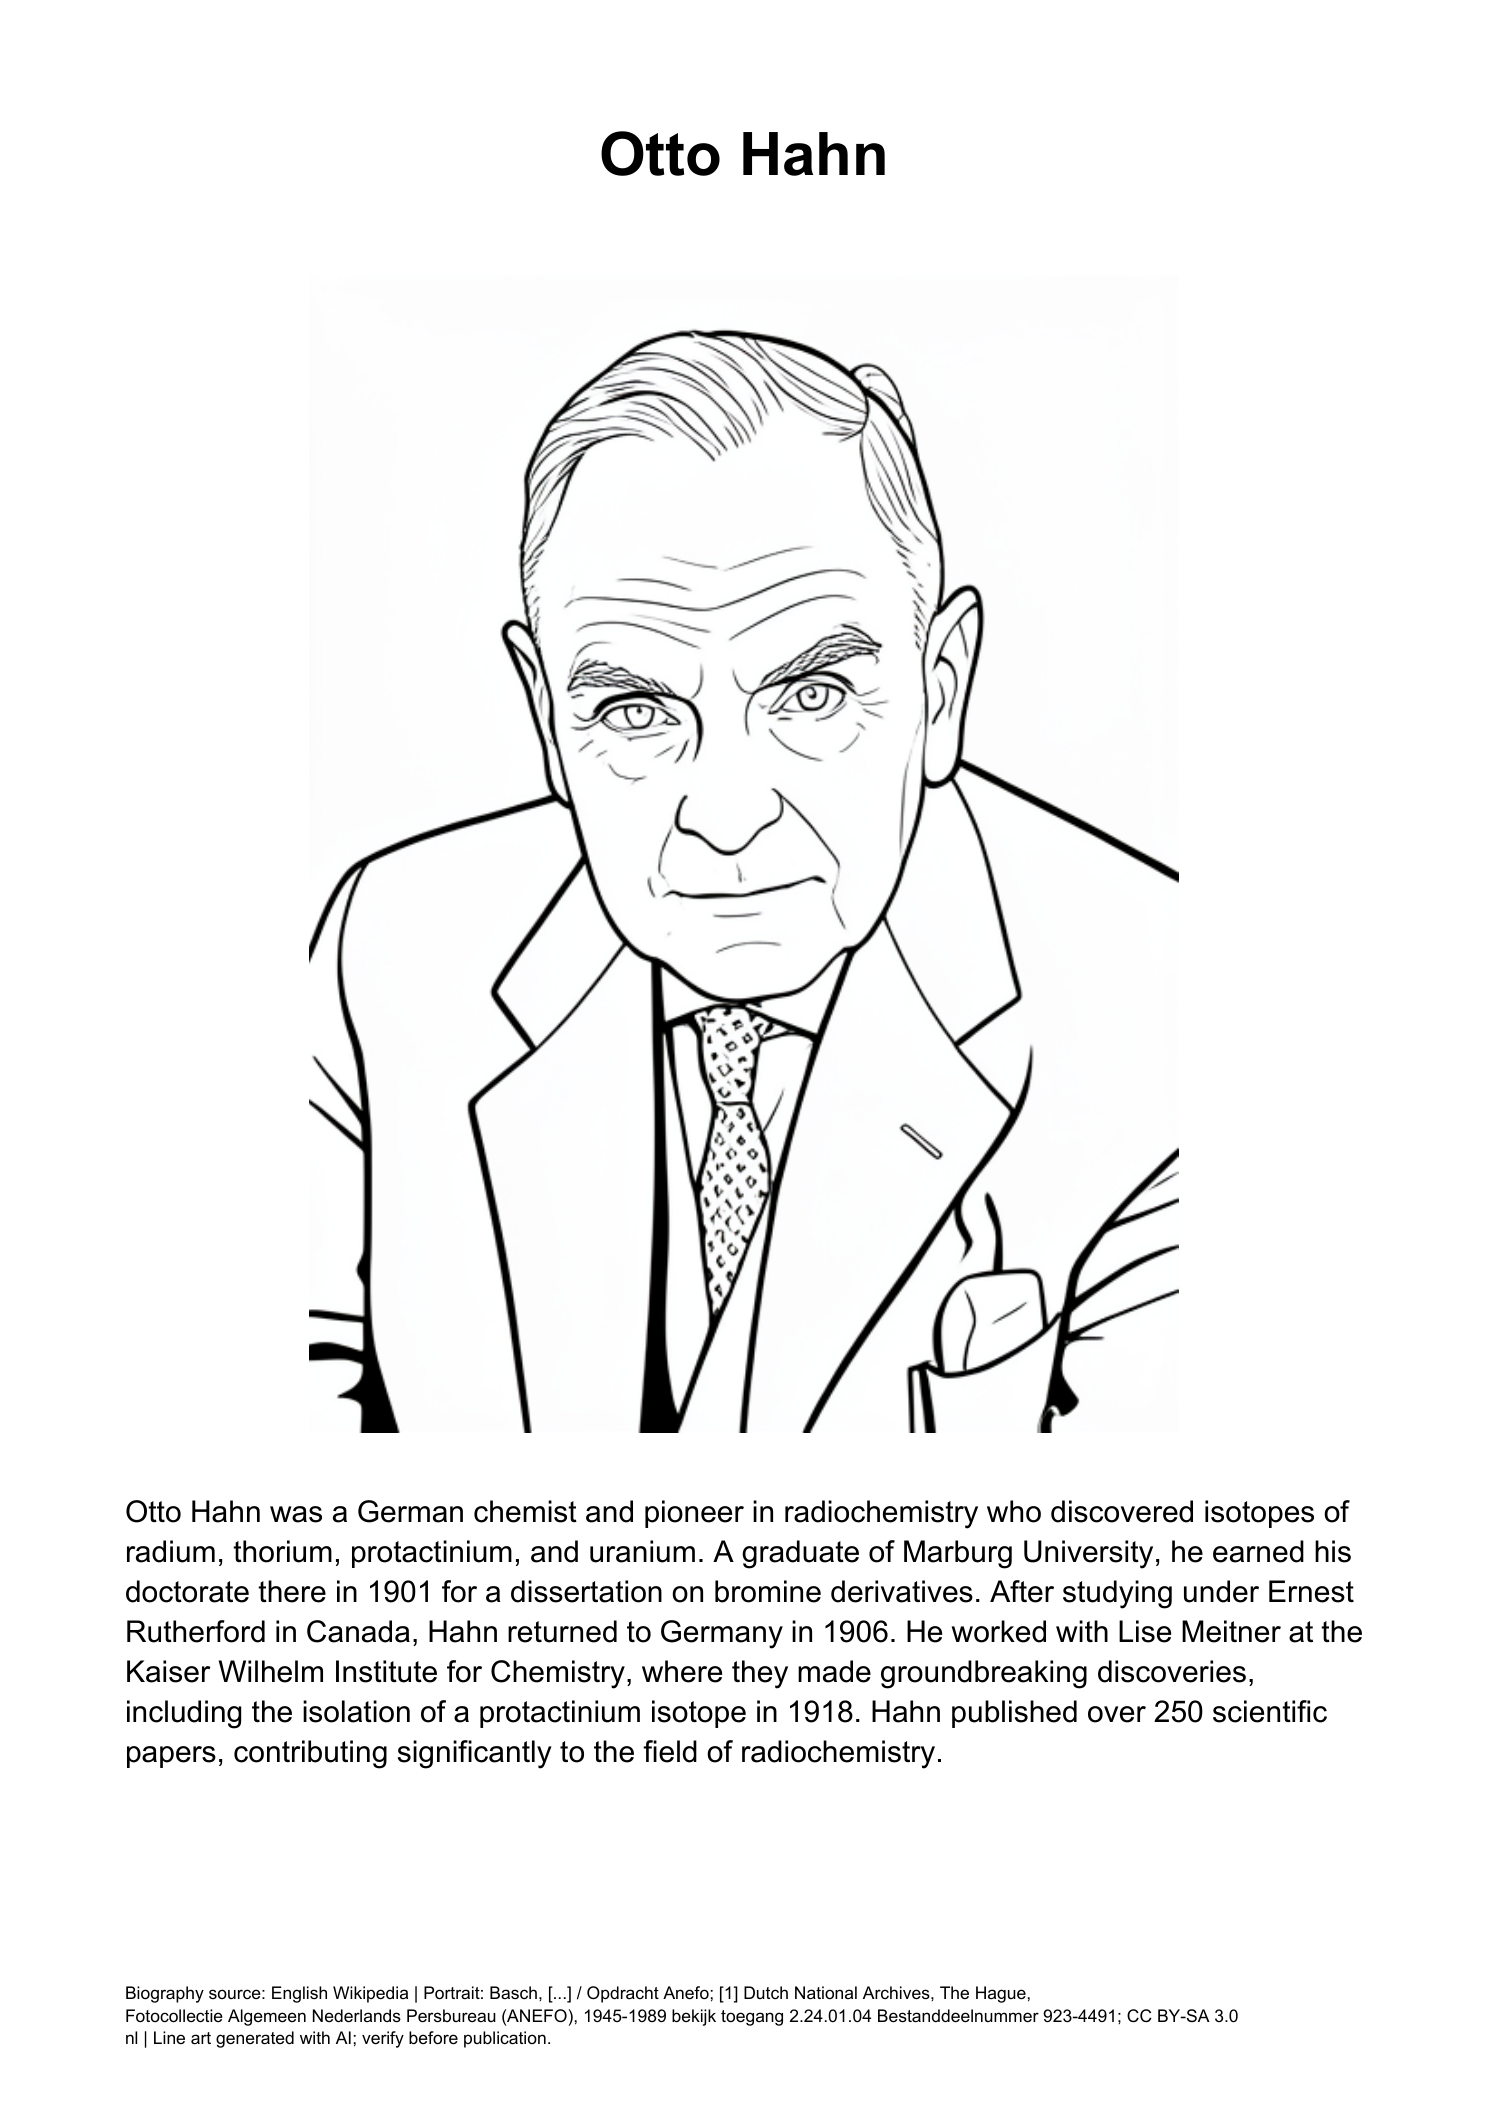
\includegraphics[width=0.93\textwidth,height=0.85\textheight,keepaspectratio]
    {figures/generated_page.png}
  \caption{The unchanged first page of the generated eight-page book,
    featuring Otto Hahn, the first current subject. The complete original
    page was mechanically rendered at 180 dpi and scaled for presentation;
    its biography, portrait, layout, source link, and attribution remain as
    generated. It is an illustrative document output, not a manually polished
    educational page or evidence of human preference.}
  \label{fig:unedited-book-page}
\end{figure*}

\end{document}
